% Two layers of a binary MERA on eight sites.
%
% Read upward. The disentanglers u act first, on pairs that straddle the
% blocks the isometries are about to join -- (2,3), (4,5), (6,7) -- and
% remove the entanglement across those block boundaries. Then each isometry w
% takes a block of two sites to one, and the next layer does the same on the
% four sites that are left: one disentangler across the middle, two isometries,
% and the two coarse-grained sites at the top are the open indices.
%
% Every index here is placed by one rule: two tensors of different extent
% meet once, in the middle of the sites they share. So a disentangler of the
% second layer, four sites wide, meets the isometries under it at their apexes,
% and an isometry of the second layer meets the disentangler it overlaps by
% half in the middle of that half. The layers are `apart': nothing joins two
% tensors side by side.
\documentclass[border=4pt]{standalone}
\usepackage{amsmath,amssymb}
\usepackage{tikz-tensors}
\input{notation}
\begin{document}
\begin{tikzpicture}
  \tnstack{M}{8}{w2, u2, w1, u1}
  \tnlayer{M}{w2}{iso/$w$/4, iso/$w$/4}
  \tnlayer{M}{u2}{., ., gate/$u$/4, ., .}
  \tnlayer{M}{w1}{iso/$w$/2, iso/$w$/2, iso/$w$/2, iso/$w$/2}
  \tnlayer{M}{u1}{., gate/$u$/2, gate/$u$/2, gate/$u$/2, .}
  \tnconnect[apart={w2, u2, w1, u1}]{M}
  \tnopen{up}{M-w2-1, M-w2-5}
  \tnopen{down}{M}
\end{tikzpicture}
\end{document}
